%!TEX root = thesis.tex
\section{Introduction}
\label{s:Introduction}

\subsection{Microrobots}
From the research and advances in recent years in the area of miniature robots used in the medicine, it is not only clear that this industry always aims for minimally invasive procedures, but also, that a surgeon's technical skills can be delegated to appropriate technologies to improve precision and dexterity \cite{Hamdorf2000a}. Wireless microrobots could perform complicated to nearly-impossible tasks and have the potential of improvement various medicinal areas \cite{Nelson2010}. Although this is a field that is mostly under development, it has been advancing very fast in the past decade \cite{Joseph2005}, \cite{Nelson2010}.

The main advantage of wireless microrobots is the fact that many locations within the human body are available for intervention \cite{Kassim2006}, \cite{Menciassi2007}. With a dimension of only a few millimeters or less, microrobots enable intervension with little trauma in areas like the central nervous system, the urinary system, and the circulatory system \cite{Nelson2010}. However, there are several constraints on the development of their developments. As objects are scaled down, the generation and storage of power becomes more complicated. Also, volumetric effects like inertia and weight lose relevance in front of viscosity and electrostatics \cite{Purcell1977}, \cite{Wautelet2001}. The approaches taken at traditional robotics is therefore completely different as the one taken for  the design and fabrication of microrobots, which relies mostly on simulations for the design and experiments for the performance \cite{Nelson2010}.

Various challenges also appear within the environment in which microrobots are to operate. Changes in the size of cavities as well as the material properties of the medium and the movement of it (for example the pulsating flow of blood) are factors the microrobots have to be able to negotiate with \cite{Nelson2010}. Although from an engineering point of view, the design approach is different towards existing tethered methods (e.g. catheters) \cite{Haga2004}, the advantages are vast, ranging from improved maneuverability to reach of inaccessible internal locations.


\subsubsection{Basic functionalities}

Although microrobots could potentially be able to carry out complex operations autonomously in the future, real microrobots in a near future will be expected to carry simple operations, often supervised or operated by a clinician. In the following a list will be presented showing the simple medical tasks for microrobots that could be feasible in the near future \cite{Nelson2010}.
\begin{itemize}
\item \textbf{Targeted therapy}: \\ This is concerned with the localized delivery of different forms of substances and energies. Targeted drug delivery allows to deliver drugs with increased concentrations in a specific region, not only improving the efficiency of the drug but also reducing the risk of negative side effects \cite{Nelson2010}. Brachytherapy works similar to the targeted drug delivery, but instead of drugs it transports radioactive sources or seeds to unwanted cells (e.g. tumors) killing them with the radiated energy \cite{Devlin2007}, whereas hyperthermia and thermoablation aim for the same through localized application of heat (being powered by high-frequency magnetic fields and ultrasound) \cite{Andra2007}, \cite{Kobayashi2011}, \cite{Baronzio2009}. 


\item \textbf{Material removal}: \\ If the robots are big enough, special tools can be designed for the microrobots to accomplish their tasks, whereas if the robots are smaller, they themselves will be the tools.\cite{Nelson2010} The two methods of material removal are ablation and biopsy/excision. Ablation is the removal of material from a certain surface. Microrobots could use this method for the removal of unwanted deposits (e.g. fat) from walls of blood vessels, either through direct scraping or through ultrasonic waves  created by resonating structures \cite{Tabatabaei2011}. Biopsy (or excision) is the retrieval of tissue samples from the body for external analysis or, potentially in-vivo when combined with remote-sensing technologies \cite{Nelson2010}.

\item \textbf{Controllable structures}: \\ Here the microrobots act as static devices with controllable positions. The microrobots can act, for example, as a scaffold \cite{Zhang2005} which supports frames for nerve regeneration, organ development, or blood vessel regrowth. The microrobots can also be used as stents to keep passageways open (e.g. a clogged vessel) \cite{Ormiston2009}, \cite{Lally2006} or as occlusions to block them (e.g. a vessel that nourishes a tumor) \cite{Fabbrini2006}. Another application is to use the microrobots as implants or electrodes brain stimulation \cite{Polikov2005}.


\item \textbf{Telemetry}: This area refers to the transmission of information from a specific location within the body with the help of microrobots that would be normally very difficult to obtain\cite{Nelson2010}. This is possible through various methods like ultrasound, radio waves or visible light \cite{Jepsen2002}. The applications include remote sensing and marking. Remote sensing transmits a signal that could contain information about concentrations of interest (e.g. oxygen) or other relevant information like the presence of cancerous cells\cite{Nelson2010}. Marking is the transmission of the microrobot's position within the body. When both applications are combined the localization of otherwise unknown phenomena within the body is possible (e.g. bleeding). 

\end{itemize}
\subsubsection{Application Areas}
With the mentioned functionalities and a size small enough to reach difficult places throughout the body the application areas are the following.

\begin{itemize}
\item \textbf{The circulatory system}: \\
Its main parts are the heart and the vessels used to transport the blood throughout the body. The distance between the heart and a certain given blood vessel is what actually decides its function and its material properties, since the pressure of the pulsations become less significant for the smaller, more distant vessels \cite{Nelson2010}.

\begin{figure}[ht]
	\centering
  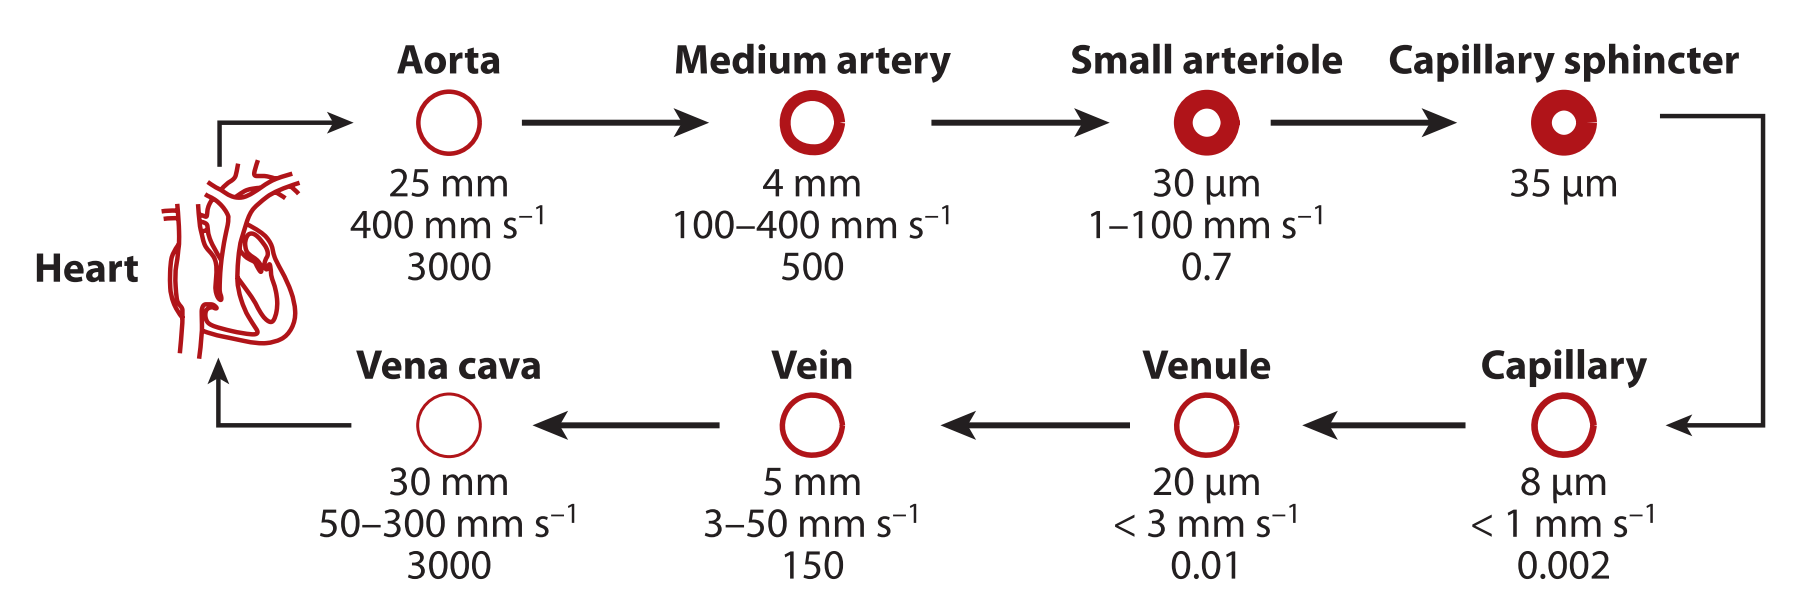
\includegraphics[width=1\textwidth]{Pictures/Bloodvessels.png}
	\caption{Vessels of the cardiovascular systems and their properties: inner diameter, average blood-flow velocity, and Reynolds number from \cite{berger1996}}
	\label{fig:veins}
\end{figure}

   In Figure \ref{fig:veins} we see the velocity and Reynolds number for the different vessel sizes. Altough blood has actually very similar intrinsic properties as those of water, the suspended blood cells create a much higher apparent viscosity as that from water. For a microrobot this could mean a very obstacle-filled working environment instead of an homogeneous liquid \cite{berger1996}. \\\\
Since almost every site within the body could be accessed through blood vessels, this could be the most important application for microrobots \cite{Nelson2010}. The most promising ones being drug delivery, removing plaque, destroying blood clots, stents or occlusions or even electrodes for electrophysiology. Some of the challenges microrobots could face tough, is the ability to swim against the flow \cite{Nelson2010}. Existing research (e.g. \cite{Cha2010}) has shown that this is indeed challenging, but possible.
\item \textbf{The central nervous system}: \\ It consists of the brain, the spinal cord, and the cerebrospinal fluid (Figure \ref{fig:nervoussystem}). The study \cite{Zaaroor2006} analyzed the geometrical and spatial characteristics of these for visualization of the spinal canal through endoscopy. These results can help set the design parameters for microrobots. Accessing the ventricles of the brain through the spine is actually possible and this would make microrobots potentially able to affect cancer therapy in the central nervous system and specifically within specific parts of the brain \cite{Nelson2010}. Injecting microrobots with a lumbar puncture would allow access to the brain for intervention, replacing invasive methods through the skull \cite{Purdy2003}. 
\begin{figure}[ht]
	\centering
  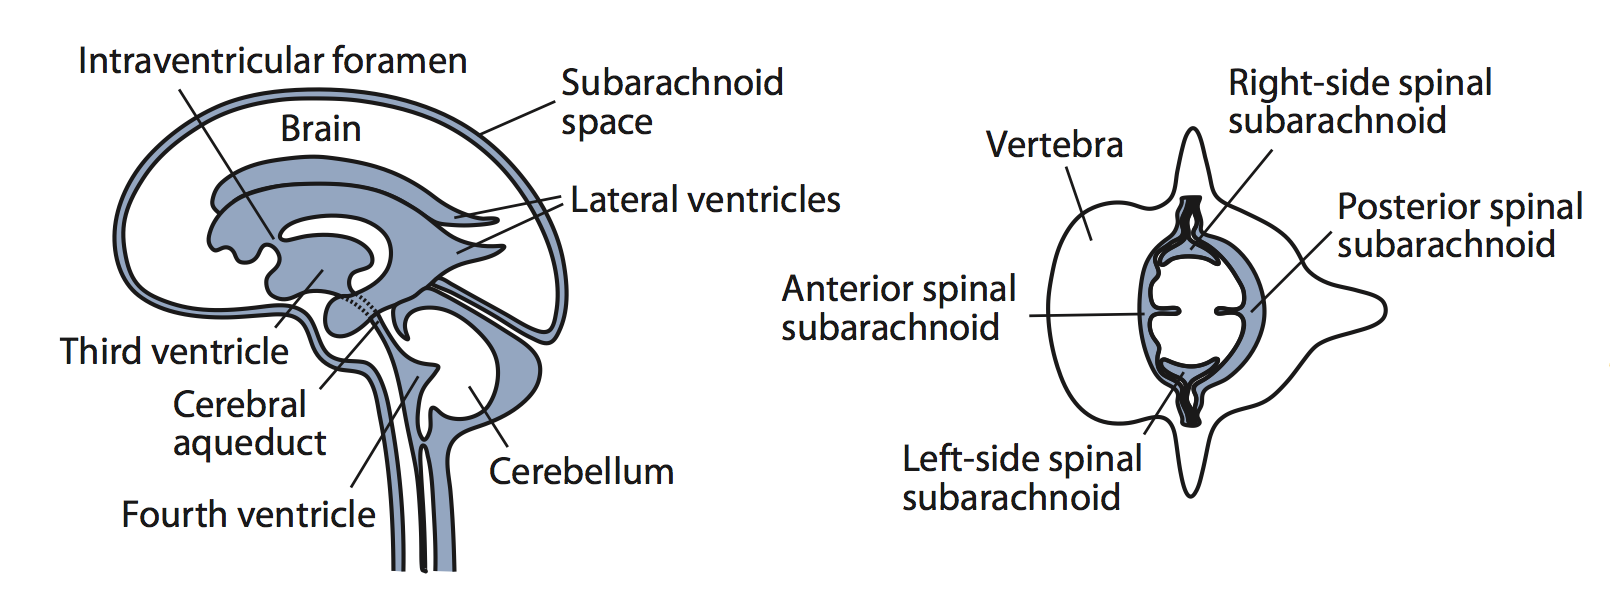
\includegraphics[width=1\textwidth]{Pictures/nervoussystem.png}
	\caption{The central nervous system, consisting of the brain and the spinal column \cite{Nelson2010}}
	\label{fig:nervoussystem}
\end{figure}
Other very important applications would be deep-brain simulation or neural prostheses, which normally would be nearly impossible since its hard reachability \cite{Nelson2010}.  Microrobots could even be used as permanent implants, but the brain's extremely delicate tissues would pose a challenge when designing them \cite{Nelson2010}.. Extensive research has been made in the field of wireless manipulation of magnetic seeds within the brain, specifically for hyperthermia methods. For more information refer to \cite{Molloy1990}.
\item \textbf{The urinary system and the prostate}: \\ This includes the kidneys, the bladder as well as the lumens connecting them and the urethra which connects the bladder to the exterior \cite{Nelson2010} (Figure \ref{fig:urinary}). 
\begin{figure}[ht]
	\centering
  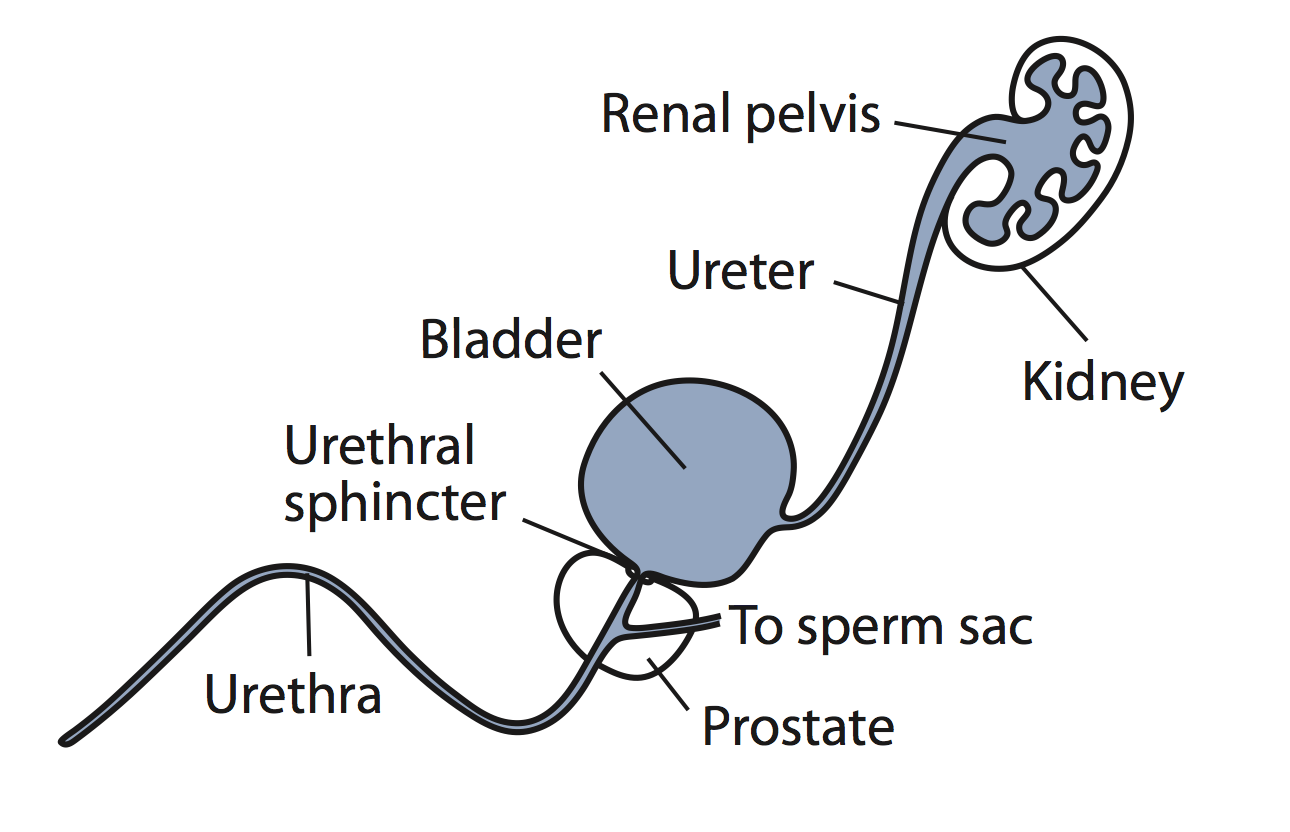
\includegraphics[width=0.5\textwidth]{Pictures/urinarysystem.png}
	\caption{The male urinary system as depicted in \cite{Nelson2010}}
	\label{fig:urinary}
\end{figure}

Microrobots operating in these areas could potentially improve the therapy of kidney stones without having to make any puncture on the kidneys which is usually related to cases of infection and blood loss \cite{Renner1999}. The methods used until now on tethered and implanted MEMS devises of urology \cite{Kristo2003} could be attached to wireless microrobots. Another possible application would be in the field of prostate cancer treatment. The most common methods used until know involve needle insertion through the perineum or through the colon, which involve the risk of damage to nerves and very complex maneuvers, respectively; microrobots would allow a minimally invasive access to the prostate through the urethra \cite{Nelson2010}. 
\item \textbf{The eye}: \\ The vitreous humor within eye is made of complex tissues that, although might be composed by mostly water, contain collagen fibrils that give viscoelastic properties and make it more of a soft tissue than a liquid \cite{Nelson2010}. The application of microrobots on the retina is where they have the most promising future, since it plays an essential role in the sight and it is very hard to access. Retinal surgery is strongly constrained by human performance \cite{Jagtap2004}, \cite{Balicki2010} and the forces needed are beyond human perception \cite{Gupta1999}, \cite{Iordachita2009} so the procedures are very risky. Microrobots would allow procedures without having to perform vicrectomy (removal of the vitreous humor) reducing the invasiveness and improving the results in the recovery \cite{Nelson2010}. The most promising application for microrobots would be diagnosis of retinal health as well as therapies for retinal vein occlusions and detached retinas, among others. There is extensive research on microrobots for intraocular procedures. For more information, refer e.g. to \cite{Yesin2006}, \cite{Ergeneman2008}, \cite{Ergeneman2008a}, \cite{Dogangil2008} and \cite{holligan2003}.
\item \textbf{The ear}:\\
The ear consists of the cochlea and the semicircular canals. It is then in this part, the inner ear, where microrobots have potential applications \cite{Nelson2010}. Through electrode implants within the cochlea that can stimulate the hearing nerve, hearing can be restored \cite{Cosetti2010}. However, the procedures are risky in terms of infections, trauma and even paralysis \cite{Stratigouleas2006} so there is still great potential for improvement through microrobots. Since the cochlear hair cells are respoinsible for natural hearing, there is extensive research around the stem-cell used for generation of these hairs. Microrobots could be used to transport and deliver the stem cells to the inner ear. For more information, refer to \cite{Parker2004} and \cite{Gunewardene2012}
\item \textbf{The fetus}: \\ Surgical procedures in a fetus can be very difficult since they are very invasive for both the mother and the fetus itself. However, open surgery can not only prevent death, but also have positive consequences for correcting impairments or malformations \cite{Flake2003}, \cite{Durkin2009}. Since they are lots of constraints in terms of dimensions and degrees of freedom of the tools that can be used, the use of microrobots have big potential of assisting these procedures \cite{Flake2003}, \cite{Berris2006}. A microrobot could perform tasks to treat cases of malformation through ablation or even act as a temporary tracheal occlusion against the pathological growth of the fetus's lungs \cite{Nelson2010}.
\end{itemize}

\subsection{Powering Microrobots}
The first challenge when designing microrobots is selecting a suitable source of power so that the locomotion can be achieved; compared to traditional robotics, there are many more limitations and constraints and we have to stick to the methods available to store, transmit and harvest power that are practically possible at the microscale \cite{Nelson2010}.

\subsubsection{Onboard scavenged power}
An feasible approach of providing a microrobot with power is with batteries; however, although these might be inexpensive, the amount energy they can provide scales with their volume, which makes them unsuitable \cite{Nelson2010}. Thin-film batteries, which use semiconductor technologies to operate, differ from traditional forms of batteries and could therefore be implemented on microrobots \cite{Nelson2010}. \\\\
Another relevant technology are MEMS-based generators. These have higher energy densities compared to batteries and traditional generators \cite{Jacobson2003}. There is also various studies that propose transducers that generate electrical energy out of different types of energy like chemical fuels, vibrations or temperature gradients \cite{DiSalvo1999}, \cite{kasap2006}. Biofuel cells, which operate at temperatures and pH similar to the ones found in the human body, would exploit the glucose and oxygen found in blood \cite{Bullen2006}, \cite{Barton2004}. Using muscle cells could be also used as actuators on micropillars \cite{Morishima2006}, cantilevers \cite{Kim2008} and other microscopic devices \cite{Xi2005}. Other possible methods of propulsion of microrobots is through the use of living microorganisms like magnetotactic bacteria, which respond to external magnetic fields \cite{Martel2009}. 

\subsubsection{Transmitted Power}
The alternative to power generation or storage implemented directly on the microrobot is the wireless transmission of energy to the device from an external source; the easiest method of doing this is using magnetic fields \cite{Nelson2010}. One method uses quasi-static or low-frequency magnetic fields that apply forces and torques directly on magnetic materials. The second method uses fluctuating magnetic fields to induce electricity. Studies \cite{Collins2002} and \cite{Siauve2003} show that, compared to electric fields, the magnetic permeability of the human body is practically the same as that in vacuum, which means that the body doesn't react to magnetic fields (i.e. magnetic transparency) and magnetic fields are therefore harmless. It is important to notice, that time varying fields do generate electrical field which could have as a consequence the cardiac fibrillation as a consequence of the stimulation of cardiac nerves. For more information about the risks and the recommended values of magnetic field and its time variation refer to \cite{Andra2007a}.

In the following, we will go in detail with the two mentioned methods of power transmission:

\begin{itemize}
\item \textbf{Induction}: \\ Using Faraday's Law of Induction we can understand this phenomenon:

\begin{equation}
V = -\frac{\textrm{d}}{\textrm{d}t}\int\limits_S \textbf{B}\cdot \textrm{d}\;\textbf{S}
\end{equation}
Here is $V$ the voltage created on a circuit by a time-varying flux of magnetic lines $\textbf{B}$ through the enclosed surface $\textbf{S}$. Usually the inducted electricity, which creates a magnetic field itself, has an effect on the circuit which created the original magnetic field $\textbf{B}$. The electricity which creates the original magnetic field is usually sinusoidal and the transfered power is optimizable (refer to \cite{bansal2006} and \cite{Theodoridis2005} for more details), but there are safety constraints that have to be taken in consideration. \\\\
Altough these methods are used in many devices \cite{Theodoridis2005}, \cite{Protection1998}, \cite{Lenaerts2007}, at the microscale there are design constraints when fabricating the small embedded coils. Also, the rectification of the voltage transmission becomes more important for microdevices since the voltage amplitudes decrease when the size decreases.

\item \textbf{Magnetic force and torque}: \\ Here the main principle is to generate mechanical energy directly on the microrobot out of magnetic fields. This is achieved by applying forces and torques directly on the magnetic materials of the microrobots. Equations ... and ... show how magnetic force and magnetic force are created from a magnetic field $\textbf{B}$:
\begin{equation}\label{eq:magdiptorqueint}
\textbf{F} = \int\limits_V(\textbf{M}\cdot\nabla)\textbf{B} \: \mathrm{d}V
\end{equation}
\begin{equation}\label{eq:magdiptorqueint}
\textbf{T} = \int\limits_V\textbf{M}\times\textbf{B}\: \mathrm{d}V + \int\limits_V \textbf{r}\times (\textbf{M}\cdot\nabla)\textbf{B} \: \mathrm{d}V
\end{equation}
where $V$ is the magnetic volume $\textbf{M}$ is the magnetization and $\textbf{r}$ is the distance from the gravity center of the body. For more details about the theory to magnetism please refer to Section (...). For small volumes, the external applied magnetic field can be modeled as uniform across the magnetic volume \cite{Nelson2010}. The magnetization usually varies throughout the body, but the average magnetization is used since the body is small \cite{Nelson2010}. Here, the strength of the forces and torques are proportional to the external field, the magnetization and the magnetic volume. \\\\
Ferromagnetic materials which exhibit a saturation magnetization and a hysteretic behavior, can be classified as either hard or soft, depending on how significant the hysteretical behavior is. Soft magnetic materials have no memory, and return to a non-magnetized state, when the applied field is removed, whereas hard magnetic materials exhibit a remanent magnetization after the applied field is no longer there \cite{Nelson2010}. \\\\
The magnetic effects on a certain body depends not only on its material properties, but also on its shape. Also, some directions within a certain shape are easier to magnetize than others. Understanding the fields that are required to control a permanent magnet wirelessly is relatively easy since the magnetization can be modeled as constant. However, for soft magnetic bodies much more complex analytical models are needed. Accurate models exist for real-time control of soft-magnetic axially symmetric bodies (beads, cylinders, ellipsoids) \cite{Abbott2007c} or bodies made out of thin planar parts \cite{Nagy2008}.\\

Soft magnetic bodies are easier to fabricate than permanent magnets, but most of the research deals with the modeling of soft magnetic bodies when they are saturated and the magnetization is near constant throughout the body. In cases where the soft magnetic body cannot be saturated, permanent magnets tend to be easier to deal with since there is little research on low-saturated cases \cite{Nelson2010}.
\end{itemize}

\subsection{Locomotion}
To be able to move a microrobot within the body energy should be transformed into movement. The material properties of the medium the robots are supposed to swim in, as well as the scale of the robots are very important. Choosing the right methods that best suit these properties is therefore essential. \\\\
The material properties of the medium are responsible for viscous forces, whereas the shape and size of the microrobot is responsible for the inertial forces. For a certain problem setting, we can calculate the corresponding Reynolds number, which is the ratio between viscous and inertial forces \cite{Purcell1977}. Since usually this number is used to compare similar geometries that only have different scales or swim in different mediums we only need a characteristic length $L$ within our geometry. Knowing the free stream velocity $v$ of the medium in relation to the robot, and the viscosity $\eta$ and $\rho$ of the medium, the ratio is calculated with the following formula:

\begin{equation}
\mathrm{Re} = \frac{\rho v L}{\eta}
\end{equation}

The Navier-Stokes equation describes the dynamics of any fluiddynamical phenomenon. If we nondimensionalize this equation we see the Reynolds numbers explicitly:

\begin{equation}
\frac{\rho v L}{\eta} \frac{\mathrm{d}}{\mathrm{d}t}\textbf{V} = - \nabla p + \nabla^2\textbf{V}
\end{equation}

Where $\textbf{V}$ is the velocity of the fluid and $p$ the pressure. If the fluid is very viscous, the free stream, the velocity very small, or the shape of the robot very small, the Reynolds number will be also very small, such that only viscous effects are of importance. The Navier-Stokes equation then simplifies then to: 

\begin{equation}
0 = - \nabla p + \nabla^2\textbf{V}
\end{equation}

Which is called a Stokes-Flow (for more details refer to  \cite{Purcell1977}). In this regime, turbulence will not happen and the flow pattern wont change much if the body moves slow or fast. A reciprocal movement (consisting of two movements that are the reverse of each other in time) will result in a negligible net movement. Usually the assumption of an open fluid is used in analytical models, but there are methods that take in consideration the effect of nearby walls \cite{Nelson2010}.\\\\
Many design methods for microrobots have been inspired by nature. Microorganisms have developed various ways of swimming at low Reynolds Number, which are completely different than the ones used by non-microscale animals \cite{Vogel2003}. Bacteria and other moving cells use non-reciprocal movement methods using different types of flagella that swim through the fluid causing propulsion. Three important methods are discussed in the following.


\subsubsection{Pulling with Magnetic Field Gradients}
This first method, is not very concerned with the details of form and locomotion of the microrobot. This principle uses the fact that, as seen in Equation (\ref{eq:magdiptorqueint}), a force can be generated out of the gradient of a magnetic field acting on a magnetized body, a method that has been used in medical application for a long time \cite{Gillies1994}. \\\\
Theres a variety of methods to create magnetic fields. The first method uses current controlled electromagnets that are positioned simultaneously. Successful implementation of this method in medical application has been seen \cite{Grady1990}.  A study \cite{Yesin2006} was also made with the overlapping of two uniform fields created by a pair of coils, then the gradient is created with a second pair of coils. Through positioning of these coils, the magnetic microrobot can be manipulated. The second method uses stationary electromagnets that are also current-controlled. In \cite{Meeker1996} three pairs of coils were positioned orthogonally in a helmet-like fashion to control the magnetic field within the human head. Another possibility is to control ferromagnetic beads with the coils used in an MRI system \cite{Mathieu2006}. The third method uses permanent magnets which is used to position magnetic-tip catheters \cite{Stereotaxis2008}. \\\\
References \cite{Nagy2008} and \cite{Abbott2007c} show analytical models for the magnetic force and torque on soft axially symmetric bodies and assembled-MEMS bodies. The advantage of these over magnetic beads is the ability to magnetize easily thanks to their strong shape anisotropy. Their shape allows them to saturate with much lower applied fields than with the beads \cite{Nagy2008}, \cite{Yesin2006}, which makes wireless control more feasible. \\\\
Locomotion achieved through the force generated by magnetic field gradients has no analogy in nature. Which could mean that is a method more effective than the mechanisms nature has developed through natural selection. It has been shown, however, that microrobots that use elastic-tail or helical propulsion are much more promising for medical applications \cite{Abbott2010}. This is because the decrease in maximum speed and force generated through gradients decay much faster when scaling down than with helical and elastic-tail propulsion and also because its easier to project magnetic fields than gradients over long distances. 

\subsubsection{Traveling-Wave Propulsion}
This method is inspired by the eukaryotic flagella. It works by the principle of traveling waves along a flexible tail, which is a non-reciprocal movement and therefore suitable for low Reynolds numbers. Although it may be a very effective movement \cite{Behkam2006}, creating this type of movement in a microrobot, as well as its control and fabrication is very difficult.\\\\
In \cite{Kosa2007} a method of constructing this propeller through piezoelectric materials is proposed. This consists of using two layers of piezoelectric actuators that make the propeller bend when one is put in tension and the other one in compression. Through alternating this mechanism one can simulate a traveling wave. The larger the number of piezoelectric actuators the better does the movement approach the one of the flagella. \\\\
Another method uses both magnetic fields and electrical power \cite{Kosa2008}. Different current-controlled coils are distributed throughout the propeller. Magnetic fields are created with the mentioned coils, which will try to align with an external applied field. Through controlling of the currents in the coils, a traveling wave can be created. This has the potential of being powered by an MRI system.\\\\
When using an elastic tail, one can imitate quite accurately the movement of the flagella only with a single actuator (acting like a whip). The disadvantage is that the efficiency is not as high as with the methods presented above. The main problems that can arise with propellers of the types mentioned here is that a very short rigid propeller, will do a reciprocal motion, whereas a long one, although approaching a perfect traveling wave, will generate a much higher drag force \cite{Nelson2010}. \\\\
The final method of propulsion is through the implementation of a chain of paramagnetic beads to form an artificial flagellum \cite{Dreyfus2005a}. An oscillating field can induce then a wave motion in the chain. Additional analysis of this swimming method has been analyzed in detail in \cite{Roper2006}, \cite{Gauger2006} and \cite{Roper2008}. The drawback here is that a body is needed where the chain has to be connected to, otherwise the drag of the flagellum creates a zero net movement.  
\subsubsection{Helical Propulsion}
We arrive to the final and for this thesis, the most important type of propulsion. This method is inspired by bacterial flagella, which use a rotor-like movement to create a helical movement out of a passive straight elastic flagellum. Scaling down a similar mechanism is extremely difficult, but a simplification is possible. Since we want to go deep in detail with this type of locomotion and its powering mechanism. We will dedicate a new section two it.

\subsection{Chiral magnetic nanomotors}
The propulsion of magnetic nanomotors with a chiral shape by a rotating magnetic field is the focus of modern biomedical applications. It relies on the interactions of the magnetic and dynamical characteristics and interactions of the system. The interest on them mainly relies on the fact that they are bio-inspired, remotely controlled and can be navigated in vivo to a specific location. They show immense potential in biomedical applications since they allow fuel-free and contact-free propulsion without changing the chemical properties in the medium and environment. \cite{Morozov2014a}. \\\\
Various research studies have proved experimentally possible to control magnetic helical propellers using rotating magnetic fields made out of ferro-magnetic, soft-magnetic materials \cite{Zhang2009}, \cite{Zhang2009a} or permanent-magnetic materials \cite{Honda1996}, \cite{Ghost2009} in many sizes including the microscale. A big advantage ist that the use of weak magnetic fields can be used to achieve the locomotion of ferromagnetic nanomotors \cite{Solovev2009}, \cite{Ghosh2009}, \cite{Wang2013}. These have to be previously magnetized by strong magnetic fields, creating a remanent magnetization when the field is removed and remains despite the presence of said weak rotating magnetic field. The velocities achieved by this mechanism are up to five orders of magnitude higher than those achieved using magnetic field gradients \cite{Nelson2010}. \\\\
Independently of the magnetic material used and the energy transfer to the helical propeller, there exist different ways of fabricating them. It can range from strips made out of different layers that obtain the helical form due to internal stresses \cite{Zhang2009}, \cite{Zhang2009a} to a wire being brought to a helical form \cite{Honda1996}. It has also been proved \cite{Purcell1977} that the efficiency of the helical structure does not depend on the cross-section of the helix. Also, the helical non-reciprocal form of the helix, allows us to revert the direction of motion so that both pulling and pushing actions are possible. \\\\
Although the preferred method would be using a rigid structure, one could use a fiber that twists up into the helix structure that stays until the torsion is removed, but this may result in less controllability towards rigid helices as well as the inability to perform a pulling motion, reversing the rotating direction (See Figure \ref{fig:rotatingflagella}) \cite{Nelson2010}. \\

\begin{figure}[ht]
	\centering
  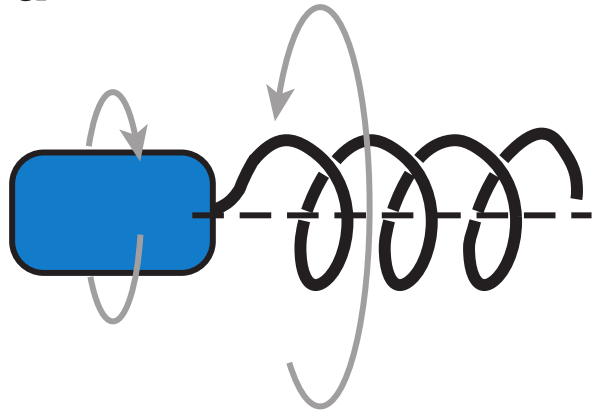
\includegraphics[width=0.5\textwidth]{Pictures/rotatingflagella.png}
	\caption{A rotary actuator turns the propeller and the body counterrotates as shown in \cite{Nelson2010}}
	\label{fig:rotatingflagella}
\end{figure}

Apart from the mentioned propulsion strategies mentioned above (rigid and non-rigid helical propulsion) there exist two other strategies for moving through lumens and soft tissue. The first one resembles more a crawling than a swimming motion. The second one involves a screw-shaped microrobot that literally screws through the medium advancing only one pitch height of the helix for one turn of it. For more information about these, please refer to \cite{Sendoh2003} and \cite{Ikeuchi1997}. In the following we will go more in detail on the methods of fabrication of these helices. 

\subsubsection{Fabrication}
The production of these structures can be achieved by various fabrication methods like ''top-down'' approach \cite{Zhang2009}, delamination of magnetic stripes \cite{Smith2011}, , glancing angle deposition \cite{Ghosh2009} as well as direct laser writing with vapor deposition \cite{Tottori2012} achieving not only the fabrication of ferromagnetic structures in the microscale but also in the nanoscale \cite{Schamel2014}.


\subsubsection{Dynamic Properties}
Independently of the strategy used from the above methods for rigid propellers we can generalize the dynamics for a movement along the helix axis. For low Reynolds number, there are linear relations between the torques and forces, and velocities, and rotation \cite{Tottori2012}, \cite{Peyer2013}, \cite{Peyer2010}, \cite{Rodenborn2013}, \cite{Behkam2006} and \cite{Abbott2010}:\\

When the torque is obtained by rotation of a magnetic field, the propulsion is fundamentally controlled by the rotation frequency of the field. The microrobot reaches an equilibrium shift of phase rotating in sync with the magnetic field . This way, the magnetic torque is in perfect balance with the torque generated by the drag forces of the medium. \\


\begin{equation}\label{eq:LinearSpeed1}
\left(\begin{array}{c}
v \\
\omega \\
\end{array}\right) =
\left[\begin{array}{cc}
a & b \\
c & d \\
\end{array}\right] \left(\begin{array}{c}
f \\
\tau \\
\end{array}\right)
\end{equation}

FIGURE 5a

It makes sense to rearrange Equation \ref{eq:LinearSpeed1}  such that the input variables are the force applied on the robot $f$ as well as the rotation frequency $\omega$ as follows:

\begin{equation}
\left(\begin{array}{c}
v \\
\tau \\
\end{array}\right) =
\left[\begin{array}{cc}
A & B \\
-B & C \\
\end{array}\right] \left(\begin{array}{c}
f \\
\omega \\
\end{array}\right)
\end{equation}

In Figure \ref{fig:LinearSpeed1}  we see the forward velocity growing linearly with the frequency until the so-called ''step-out'' frequency is reached (consistent with Equation \ref{eq:LinearSpeed1}). This is the frequency where the magnetic torque is no longer big enough to keep the structure rotating in sync with the magnetic field. Here the velocity starts decreasing significantly. Recent studies  \cite{Peyer2013}, \cite{Morozov2014} and \cite{Morozov2014a} has shown experimentally this behavior. \\

\begin{figure}[ht]
	\centering
  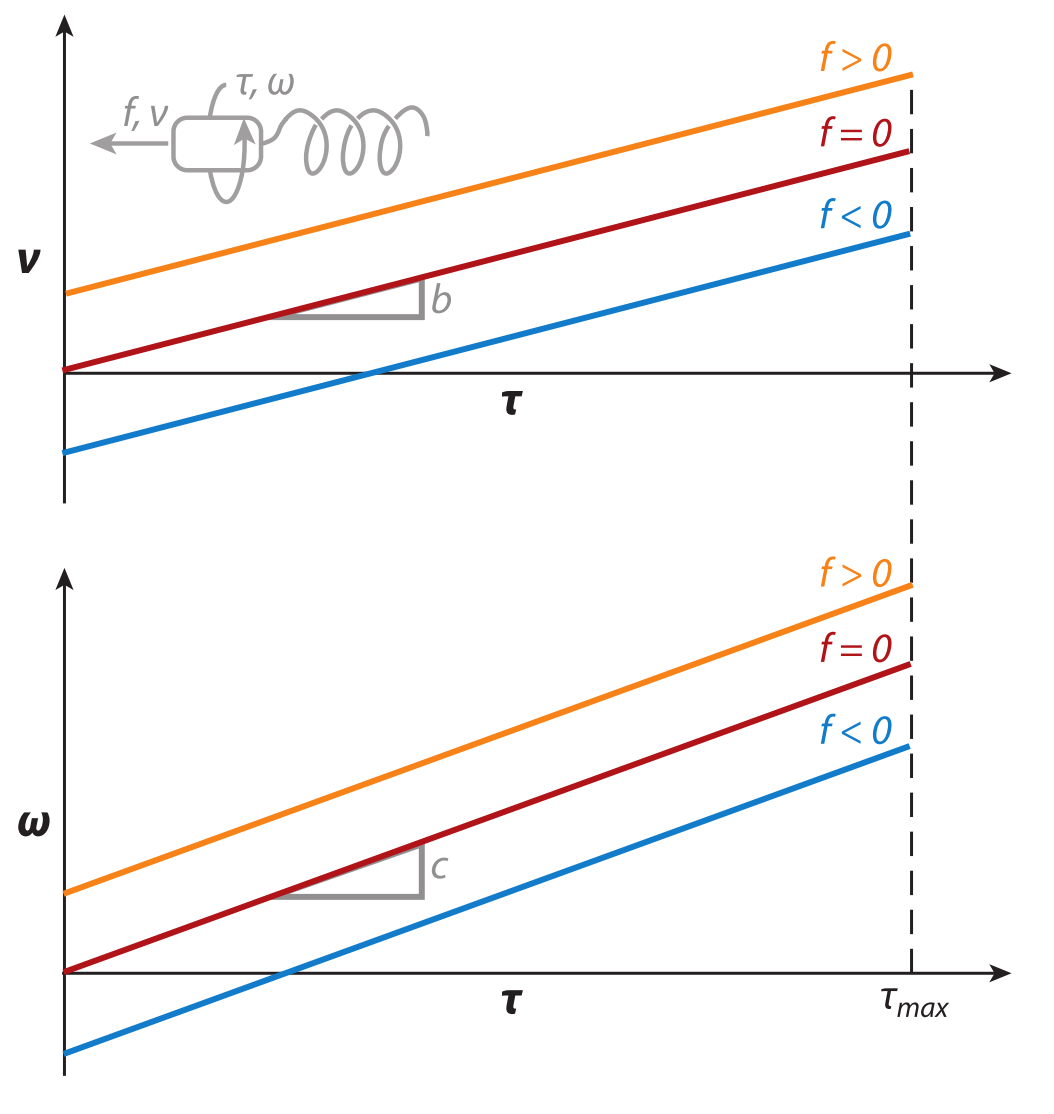
\includegraphics[width=0.7\textwidth]{Pictures/LinearSpeed1.png}
	\caption{Dynamic behaviour of helical-motors as shown in \cite{Nelson2010}}
	\label{fig:LinearSpeed1}
\end{figure}

Rodenborn did an analysis in \cite{Rodenborn2013} using the above linear model to find out the dynamic parameters $a,b,c,$ and $d$ using macroscopic swimmers in a highly viscous fluid (keeping the Reynolds number very small) and measuring the relevant dynamic variables. Comparatively numerical simulations where performed using resistive force theory of Gray and Hancock, and Lighthill, slender body theories (Lighthill and Johnson) as well as the Stokeslet numerical method. In this analysis the experimental results differ significantly from the predictions of the models used by resistive force theory, whereas the slender body and Stokeslet analyses agree with them (Figure \ref{fig:Rodenborn2013}). \\

\begin{figure}[ht]
	\centering
  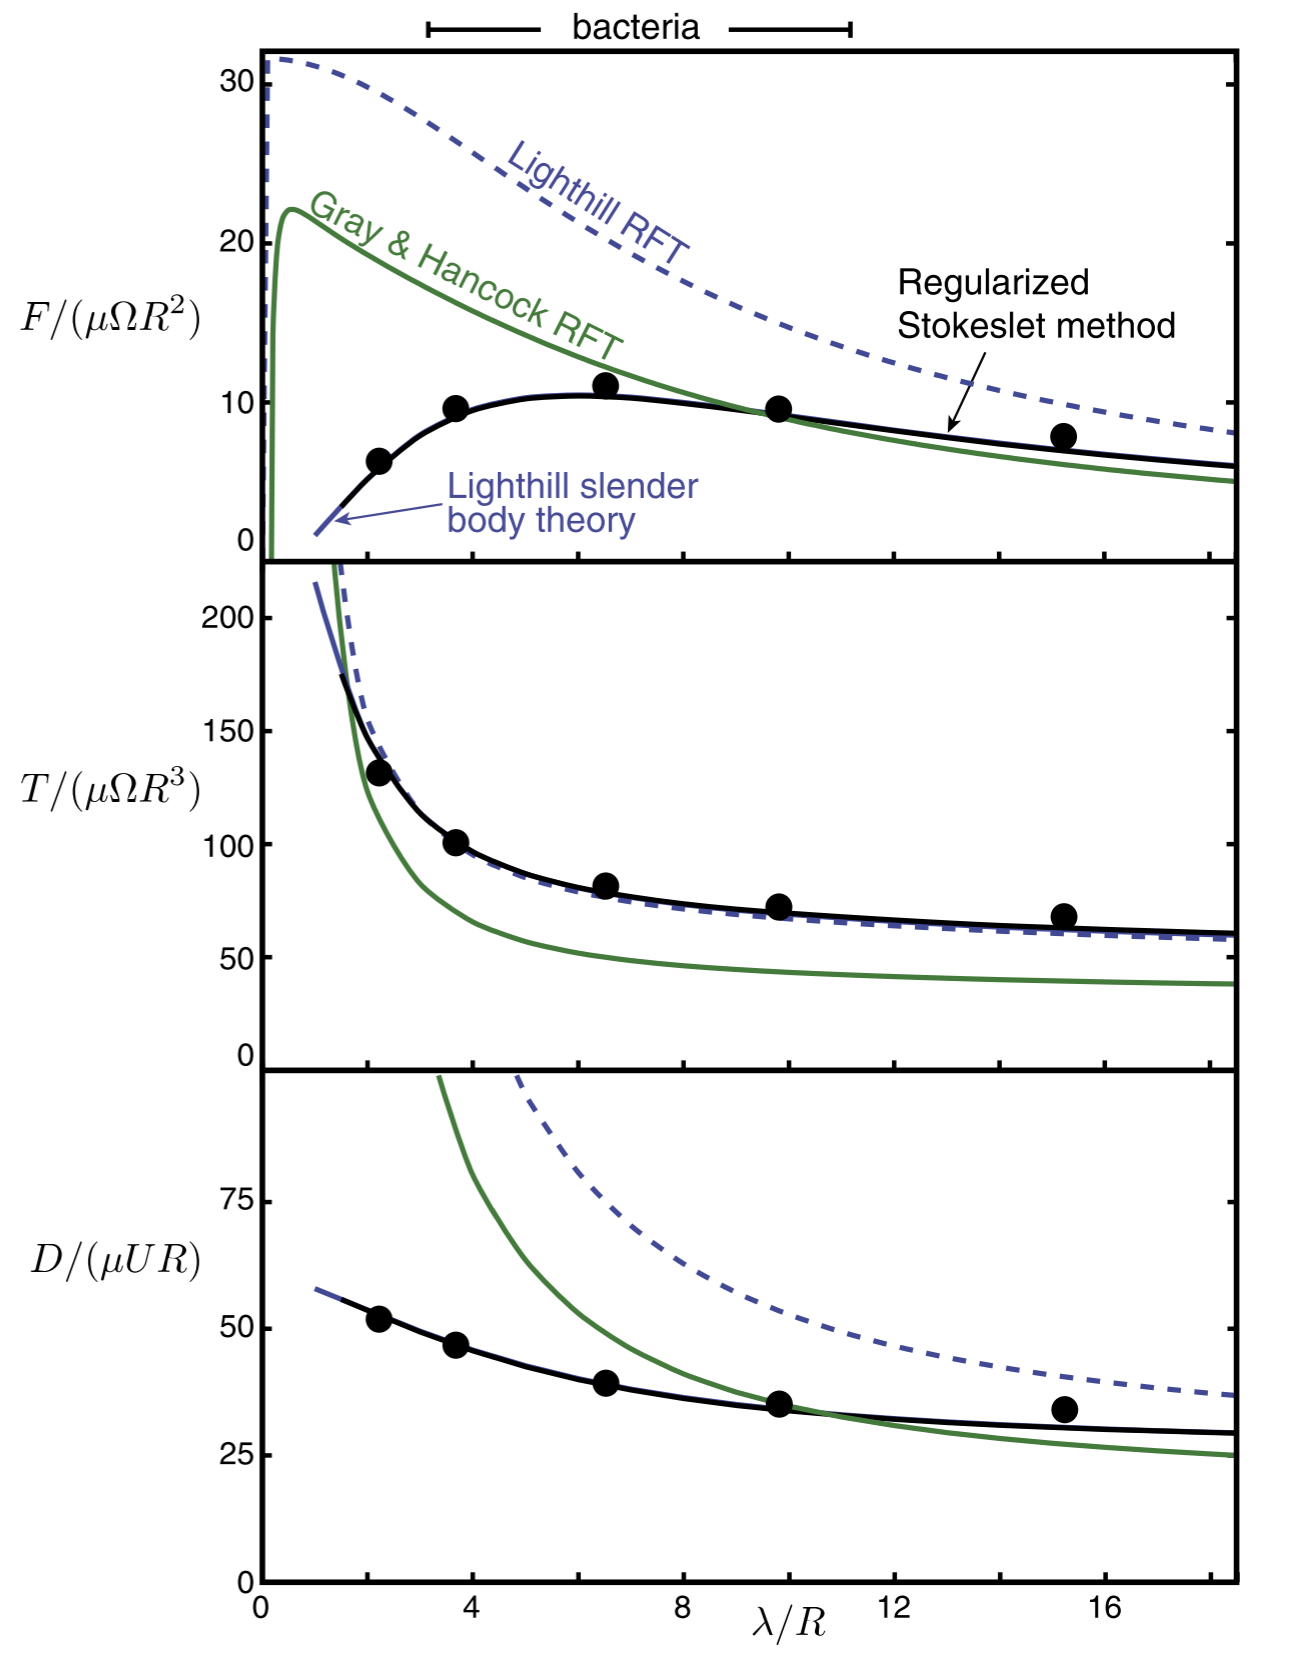
\includegraphics[width=0.7\textwidth]{Pictures/Rodenborn2013.png}
	\caption{Dynamic measurements (Thrust, torque and drag) compared to Resistive Force Theory model, Slender Body model and Stokeslet analysis for helical flagella as a function of pitch-to-radius ratio as shown in \cite{Rodenborn2013}}
	\label{fig:Rodenborn2013}
\end{figure}

\cite{Morozov2014} analyzed the different regimes when it comes to orientation and propulsion depending of the actuation frecuency. The theoretical predictions agree accurately with the available experimental data. Although in Figure \ref{fig:LinearSpeed1} the relation between propulsion speed and frequency is linear, it only holds when the helix is performing a perfect rotation along the helix axis. \cite{Morozov2014} includes the fact that a wobbling/tumbling movement is first reached until the movement stabilizes to a perfect rotation along the axis. This creates nonlinearities in the model. In Figure \ref{fig:Morozov2014a} we see this behavior. \\

\begin{figure}[ht]
	\centering
  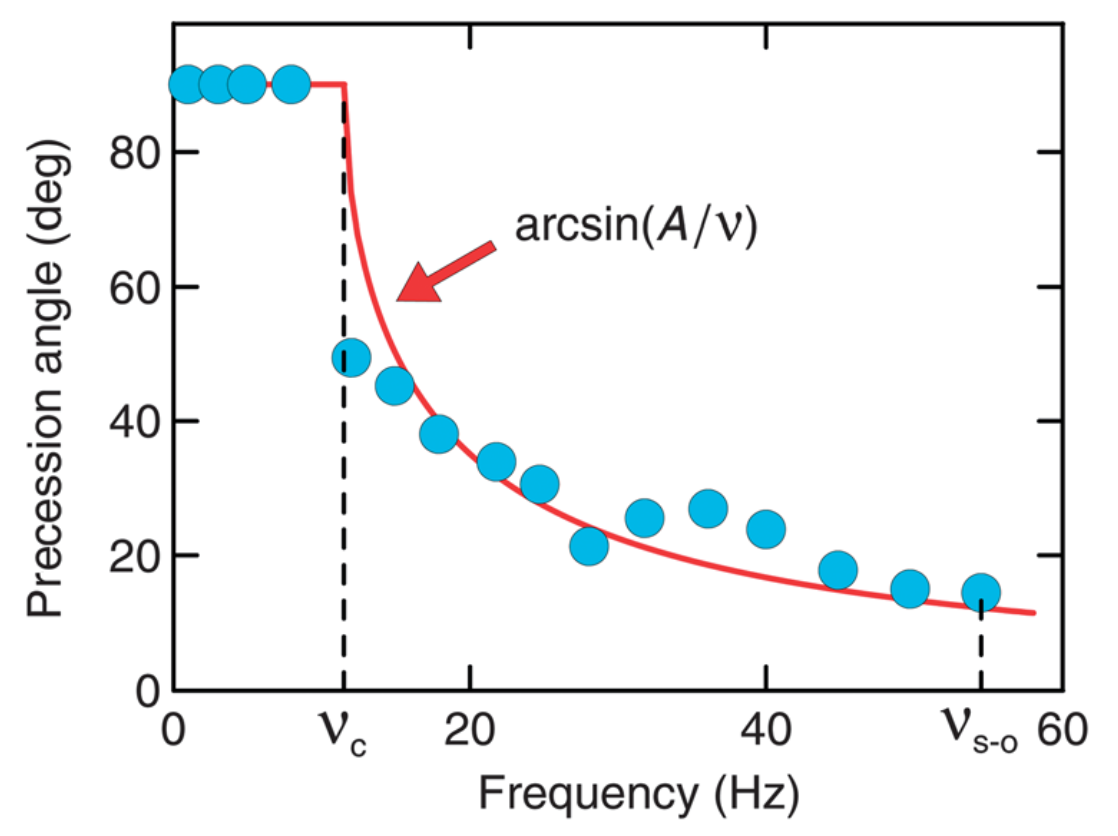
\includegraphics[width=0.7\textwidth]{Pictures/Morozov2014a.png}
	\caption{Experimental results of propulsion as a function of frequency as shown in \cite{Morozov2014}}
	\label{fig:Morozov2014a}
\end{figure}

Figure \ref{fig:Morozov2014b} on the other hand, shows how the precession angle stabilizes towards zero with higher frequencies (before the step out frequency).\\

\begin{figure}[ht]
	\centering
  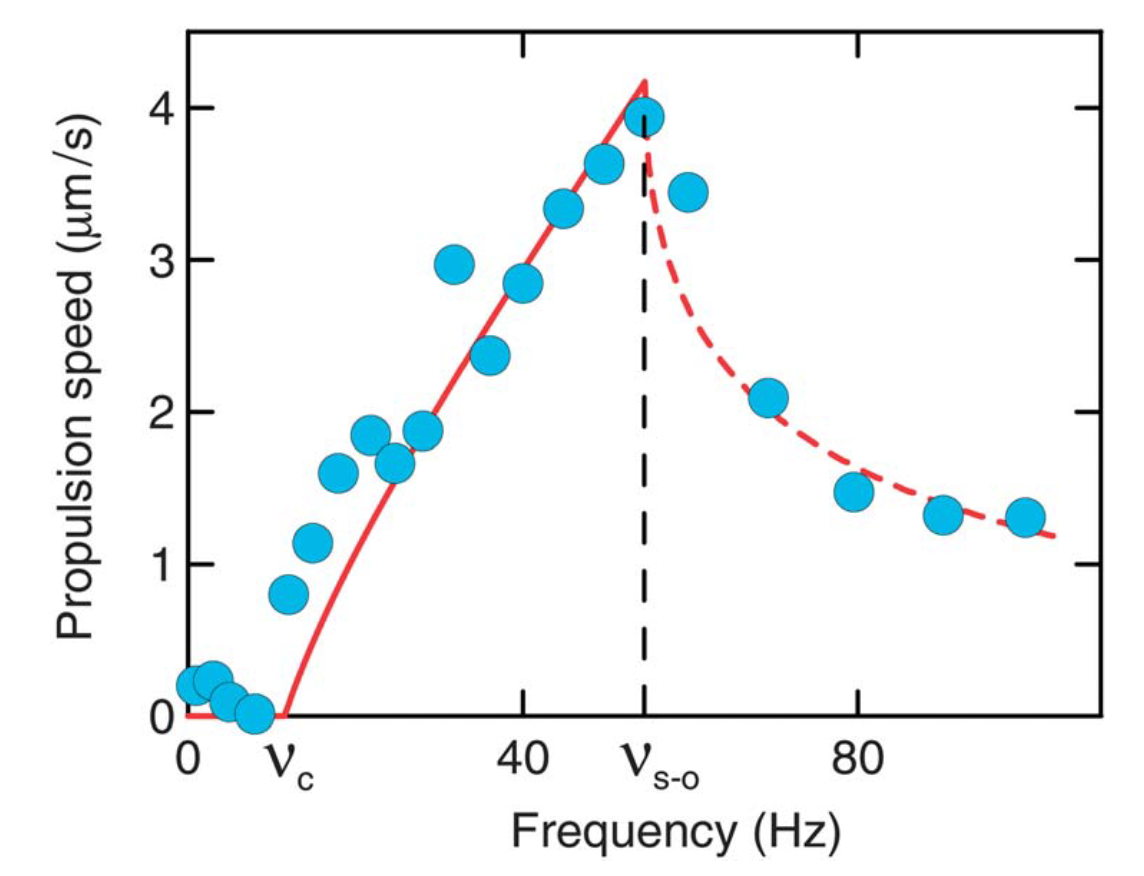
\includegraphics[width=0.7\textwidth]{Pictures/Morozov2014b.png}
	\caption{Experimental results of precession angles as a function of frequency as depicted in \cite{Morozov2014}}
	\label{fig:Morozov2014b}
\end{figure}

\subsubsection{Magnetic Properties}

As it was mentioned above. In order to achieve a more optimal propulsion, the orientation of the helix towards the axis of the rotating magnetic field (precession angle) plays an important role. Clearly the magnetic properties of the helix are crucial, specially how the body itself magnetizes in the presence of an applied field. Several studies go into this topic. \cite{Abbott2007} deals with soft-magnetic axial symmetric bodies and actually mentions that magnetization with a low applied field completely differs from a magnetization with a high applied field. \cite{Morozov2014a} analyses the alienation of the helix with a given magnetization on a given applied field. \cite{Sheka2015} goes in depth with the details of the magnetization of a helix in presence of a applied field and the effects that arise due to the curvature of the geometry.






